\documentclass[a4paper,12pt,chapterprefix=false,bibliography=totoc,listof=totoc,]{scrreprt}

% Benannte Farben
\usepackage{xcolor}
% Schriftauswahl
\usepackage{fontspec}
% Spracheinstellungen
\usepackage[english]{babel}
% Grafiken einfügen
\usepackage{graphicx}
% [H] Platzierung
\usepackage{float}
% Tabellen
\usepackage{tabu}
% KOMA-Script Mods für float,hyperref,listings,setspace
\RequirePackage{scrhack}
% hyperref als letzes
\RequirePackage{hyperref}

\hypersetup{
    colorlinks=true,
    linkcolor=blue,
    filecolor=magenta,      
    urlcolor=cyan,
}

\setlength{\parindent}{0pt}

\begin{document}
\begin{flushright}
GameBase
\\
Software Requirements Specification
% \\
% For <Subsystem or Feature>
\bigbreak
Version 1.0
\end{flushright}
\chapter*{Revision History}
\begin{table}[H]
	\centering
	\everyrow{\hline}
	\begin{tabu} to \textwidth {|X[c]|X[c]|X[c]|X[c]|}
		Date & Version & Description & Author\\
		23/10/2019 & 0.1 & Added Use Case Diagram & Norman Gehrsitz\\
		<dd/mmm/yy> & <x.x> & <details> & <name>\\
	\end{tabu}
	\label{tab:rev-hist}
\end{table}

\tableofcontents

\chapter{Introduction}
%[The introduction of the Software Requirements Specification (SRS) should provide an overview of the entire SRS. It should include the purpose, scope, definitions, acronyms, abbreviations, references, and overview of the SRS.]

% [Note: The Software Requirements Specification (SRS) captures the complete software requirements for the system, or a portion of the system.  Following is a typical SRS outline for a project using only traditional natural-language style requirements – with no use-case modeling.  It captures all requirements in a single document,  with  applicable sections inserted from the  Supplementary Specifications (which would no longer be needed).  For a template of an SRS using use-case modeling, which consists of a package containing Use-Cases of the use-case model and applicable Supplementary Specifications and other supporting information, see rup\_SRS-uc.dot.]

% [Many different arrangements of an SRS are possible.  Refer to [IEEE830-1998] for further elaboration of these explanations, as well as other options for SRS organization.]

\section{Purpose}
% [Specify the purpose of this SRS. The SRS should fully describe the external behavior of the application or subsystem identified. It also describes nonfunctional requirements, design constraints and other factors necessary to provide a complete and comprehensive description of the requirements for the software.]
The purpose of this document is to give a general description of the GameBase project. It explains our vision and all features we plan to provide. It is supposed to offer insights into the system in terms of back- and frontend, the interfaces in both ends for communication and the constraints of the system.

\section{Scope}
% [A brief description of the software application that the SRS applies to; the feature or other subsystem grouping; what Use-Case model(s) it is associated with;  and anything else that is affected or influenced by this document.]
This document is designed for internal use only and will outline the development process of the project.

\section{Definitions, Acronyms and Abbreviations}
{\color{blue} [This subsection should provide the definitions of all terms, acronyms, and abbreviations required to properly interpret the SRS.  This information may be provided by reference to the project Glossary.]}

\section{References}
{\color{blue} [This subsection should provide a complete list of all documents referenced elsewhere in the SRS.  Each document should be identified by title, report number (if applicable), date, and publishing organization.  Specify the sources from which the references can be obtained. This information may be provided by reference to an appendix or to another document.]}

\section{Overview}
% [This subsection should describe what the rest of the SRS contains and explain how the document is organized.]
The next chapters provide information about our vision based on a use case diagram as well as more detailed software requirements. Additionally, we are going to outline the steps required to comply with legal requirements and technical standards.

\chapter{Overall Description}
\section{Vision}
% [This section of the SRS should describe the general factors that affect the product and its requirements.  This section does not state specific requirements.  Instead, it provides a background for those requirements, which are defined in detail in Section 3, and makes them easier to understand. Include such items as:
% \begin{itemize}
% 	\item product perspective
% 	\item product functions
% 	\item user characteristics
% 	\item constraints
% 	\item assumptions and dependencies
% 	\item requirements subsets
% \end{itemize}]
Setting up game servers can be painful. Either way when hosting on a dedicated server, you need to get into e. g. Bash where things could get messy really fast if you don’t have enough experience. And in case you want to get rid of your installed unsteady server, you also need to take care of removing all remaining files that sit somewhere in your file system. Good luck on that!

With GameBase, we want to make your game server deployment life way easier. Using Docker – a state-of-the-art virtualisation technology – servers can be set up through templates on a website and ready to be deployed with just one click. This also makes sure that every game server is isolated from each other avoiding possible conflicts with each other as well.

\section{Product perspective}
\begin{figure}
	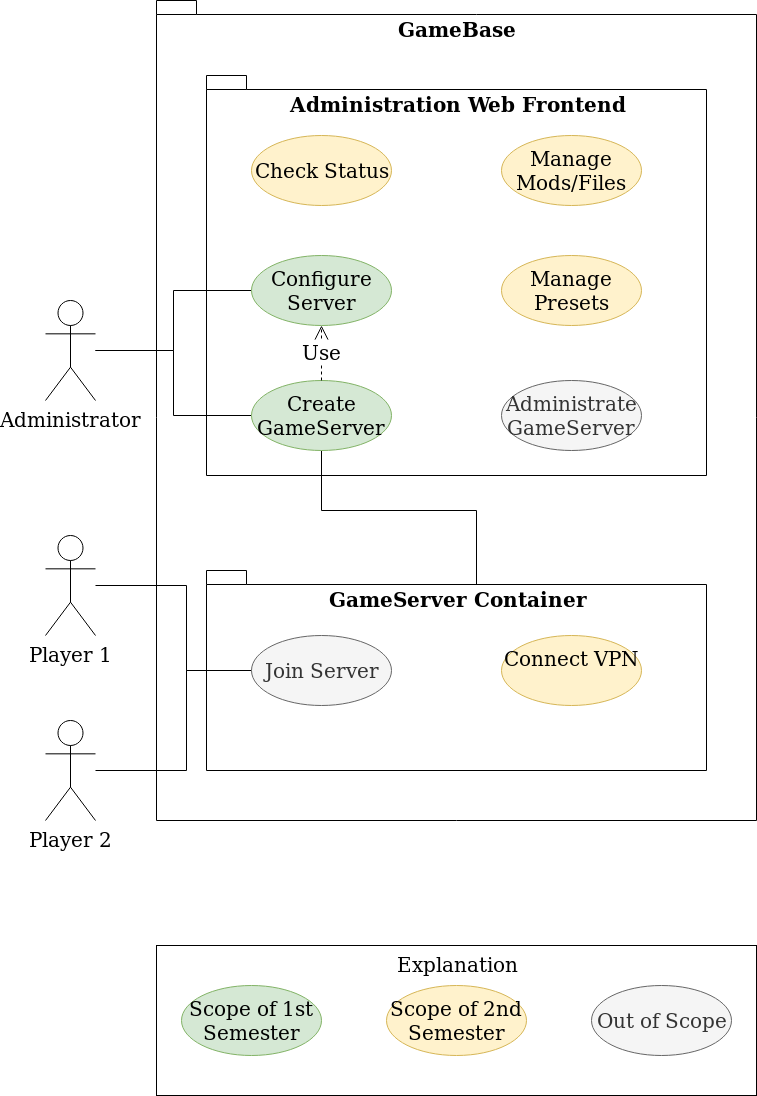
\includegraphics[width=\textwidth]{Use_Case_Diagramm.png}
	\caption{Use Case Diagramm}
	\label{fig:ucd}
\end{figure}
Players are featured in our diagram even though they are not interacting with our application directly because after all connecting to the servers is a crucial part of our system.
Administration of the game servers with game specific features like Kicking, Banning and Map Rotations is also out of scope as there are already well polished Tools for this who can work independently from our Platform.
The main use cases of our application is managing the game server containers.
As such creation and configuration of severs is the milestone for our first semester, whereas Status reporting, managing server files, enabling network access to the containers network and managing server presets is in scope for the second semester.

\chapter{Specific Requirements}
{\color{blue} [This section of the SRS should contain all the software requirements to a level of detail sufficient to enable designers to design a system to satisfy those requirements, and testers to test that the system satisfies those requirements.   When using use-case modeling, these requirements are captured in the Use-Cases and the applicable supplementary specifications.  If use-case modeling is not used, the outline for supplementary specifications may be inserted directly into this section, as shown below.]}

\section{Functionality - Backend}
{\color{blue} [This section describes the functional requirements of the system for those requirements which are expressed in the natural language style. For many applications, this may constitute the bulk of the SRS Package and thought should be given to the organization of this section. This section is typically organized by feature, but alternative organization methods may also be appropriate, for example, organization by user or organization by subsystem.  Functional requirements may include feature sets, capabilities, and security.

Where application development tools, such as requirements tools, modeling tools, etc., are employed to capture the functionality, this section document will refer to the availability of that data, indicating the location and name of the tool that is used to capture the data.]}

{\color{magenta}
The backend is needed to separate the user interface from the data storage. It verifies if the correct permissions are present to request data or to ensure that incoming data is properly parsed and saved correctly. For security reasons data is filtered by the backend. It is then packed in the right format which the next chapter describes. The data is kept inside a database and maintained by the backend.
}

% \subsection{<Functional Requirement One>}
% [The requirement description.]

\subsection{{\color{magenta} Read data given over API endpoints}}
{\color{magenta}
For the communication between both sides (frontend and backend) a universal data format is needed, therefore JSON is used. The frontend sends data in JSON to the backend in form of a request and waits for a response from the backend which also answers with JSON.
}

\subsection{{\color{magenta} Parse data}}
{\color{magenta}
For the communication between both sides (frontend and backend) a universal data format is needed, therefore JSON is used. The frontend sends data in JSON to the backend in form of a request and waits for a response from the backend which also answers with JSON.
}

\subsection{{\color{magenta} Provide data}}
{\color{magenta}
After data is requested from the frontend and the user is allowed to do so, the backend sends out the previously mentioned DTO objects. In addition, the response contains a HTTP status code even if the request failed so that the frontend knows if it just received data or an error.
}

\section{Functionality - Frontend}
{\color{blue} [This section describes the functional requirements of the system for those requirements which are expressed in the natural language style. For many applications, this may constitute the bulk of the SRS Package and thought should be given to the organization of this section. This section is typically organized by feature, but alternative organization methods may also be appropriate, for example, organization by user or organization by subsystem.  Functional requirements may include feature sets, capabilities, and security.

Where application development tools, such as requirements tools, modeling tools, etc., are employed to capture the functionality, this section document will refer to the availability of that data, indicating the location and name of the tool that is used to capture the data.]}

{\color{magenta}
The frontend provides an user interface for the users to interact with and is able to request data from the data backend. The following subsections explain the types of data the frontend can request. Each of the subsections corresponds to one or more use cases.
}

% \subsection{<Functional Requirement One>}
% [The requirement description.]

\subsection{{\color{magenta} User system}}
{\color{magenta}
At registration, the data provided by the user is stored in the backend. It is needed to log in, edit the profile and also provides the basis for a permission-system. According use cases are:

\begin{itemize}
    \item Register
    \item Login
    \item Logout
    \item Change profile
    \item Delete profile
\end{itemize}
}

\subsection{{\color{magenta} App server system}}
See use-cases:
\begin{itemize}
    \item \href{https://gamebase.pages.gitlab.tandashi.de/documentation/UCCreateGameServer.pdf}{Create Gameserver}
    \item \href{https://gamebase.pages.gitlab.tandashi.de/documentation/UCConfigureGameServer.pdf}{Configure Gameserver}
\end{itemize}
{\color{magenta}
The user interface exposes several highly abstracted options for investigating and controlling containers to users through the app server system. Users should be able to deploy containers in very few steps (ideally a single click) which can be achieved by using sane default configurations. According use cases are:

\begin{itemize}
    \item Request deployment
    \item Cancel deployment
    \item View deployment/container status
    \item View reports/logs/metrics
\end{itemize}
}

\section{{\color{magenta} Usability}}
% [This section should include all of those requirements that affect usability. For example,
% \begin{itemize}
% 	\item specify the required training time for a normal users and a power user to become productive at particular operations
% 	\item specify measurable task times for typical tasks or base the new system’s usability requirements on other systems that the users know and like
% 	\item specify requirement to conform to common usability standards, such as IBM’s CUA standards Microsoft’s GUI standards]
% \end{itemize}

{\color{magenta}
We will build the user interface intuitive, so that a new user does not necessarily need an explanation. Even if our users don't know what containers are or how they work they should be able and comfortable with the deployment. For advanced users a comprehensive documentation should be provided to enable customized deployment scenarios.
}

\section{{\color{magenta} Reliability}}
% [Requirements for reliability of the system should be specified here. Some suggestions follow:
% \begin{itemize}
% 	\item Availability—specify the percentage of time available ( xx.xx%), hours of use, maintenance access, degraded mode operations, etc.
% 	\item Mean Time Between Failures (MTBF) — this is usually specified in hours, but it could also be specified in terms of days, months or years.
% 	\item Mean Time To Repair (MTTR)—how long is the system allowed to be out of operation after it has failed?
% 	\item Accuracy—specify precision (resolution) and accuracy (by some known standard) that is required in the system’s output.
% 	\item Maximum Bugs or Defect Rate—usually expressed in terms of bugs per thousand of lines of code (bugs/KLOC) or bugs per function-point( bugs/function-point).
% 	\item Bugs or Defect Rate—categorized in terms of minor, significant, and critical bugs: the requirement(s) must define what is meant by a “critical” bug; for example, complete loss of data or a complete inability to use certain parts of the system’s functionality.]
% \end{itemize}
{\color{magenta}
In the following we describe the availability, Mean Time Between Failures and Mean Time To Repair, accuracy and bug classes we strive for.
}

% \subsection{<Reliability Requirement One>}
% [The requirement description.]

\subsection{{\color{magenta} Availability}}
{\color{magenta}
Since we want to provide hosting for our users but also allow them to host the software for themselves or using other providers, we cannot specify this requirement in great detail. Ultimately even the reliability of our own hosting option would be subject to the capabilities of our hosting provider. Due redundancy and other security arrangements, most providers can ensure an uptime of over 99.9\% which equates to approximately 8 hours per year. It is thus reasonable to assume that a sufficiently mature implementation of the software can achieve comparable reliability.
}

\subsection{{\color{magenta} Mean Time Between Failures \& Mean Time To Repair}}
{\color{magenta}
If the application fails due an hardware issue, then the mean times are up to our hosting provider. Since the ensured uptime of most hosting providers is 99.9\%, they try to fix the issue within a few minutes. However, if the application fails due a bug in our code, we can revert the code to a previous version that worked fine. This shouldn't take more than one or two hours from the point on we noticed.
}

\subsection{{\color{magenta} Accuracy}}
{\color{magenta}
The status data which is displayed to users should be as close to realtime as possible. This is because the software has to interact with live systems and we want our users to be capable of making relevant decisions at all times. The fulfillment of this requirement is likely to depend on the individual hosting solution of our users and in this case outside of our controll. Otherwise we should be able to ensure this by preferring both fast and efficient implementations and consequently, algorithms.
}

\subsection{{\color{magenta} Bug classes}}
{\color{magenta}
We classify bugs which might appear in the software into either one of these two categories:

\begin{itemize}
    \item Critical bug: A critical bug occurs when the users are not able to use the application at all. A data breach or other condition where data that is supposed to be secret becomes publicly accessible is also considered a critical bug.
    \item Non-critical bug: A non-critical bug appears when the user can use the application but it appears glitched but the user experience is just slightly impacted. Crucially, bugs in this category have minimal impact on the use cases as outlined in this specification.
\end{itemize}
}

\section{{\color{blue} Performance}}
{\color{blue} [The system’s performance characteristics should be outlined in this section. Include specific response times. Where applicable, reference related Use Cases by name.
 \begin{itemize}
 	\item response time for a transaction (average, maximum)
 	\item throughput, for example, transactions per second
 	\item capacity, for example, the number of customers or transactions the system can accommodate
	\item degradation modes (what is the acceptable mode of operation when the system has been degraded in some manner)
	\item resource utilization, such as memory, disk, communications, etc.
 \end{itemize}]}

{\color{magenta}
In general, we try to keep to user experience fluent and response times low.
}

% \subsection{<Performance Requirement One>}
% [The requirement description goes here.]

\section{{\color{magenta} Supportability}}
% [This section indicates any requirements that will enhance the supportability or maintainability of the system being built, including coding standards, naming conventions, class libraries, maintenance access, maintenance utilities.]
{\color{magenta}
Our frontend, backend and each functionality will be clearly separated and we try to stick to naming conventions which are common in the used technologies. We especially value practices which lead to the writing of clean code. By properly documenting code through comments and backing documents we make it easy to understand our infrastructure and increase maintainability.
}

% \subsection{<Supportability Requirement One>}
% [The requirement description goes here.]

\section{Design Constraints}
% [This section should indicate any design constraints on the system being built. Design constraints represent design decisions that have been mandated and must be adhered to.  Examples include software languages, software process requirements, prescribed use of developmental tools, architectural and design constraints, purchased components, class libraries, etc.]

% \subsection{<Design Constraint One>}
% [The requirement description goes here.]
 
\subsection{{\color{magenta} Usage of Software languages and frameworks}}
{\color{magenta}
For the clientsided frontend we will use a mix of HTML, CSS, JavaScript and the ReactJS Framework. ReactJS helps building interactive UIs that can be updated dynamically and therefore eliminate the need to refresh the web application. One can also develop single components and can reuse them all over the application. Such a component could be a login form, a profile card or anything else one wants to reuse. We are going to import a React framework called Material-UI that provides a lot of pre-defined components based on the Material Design Specification. The development will take place with the newest version of JavaScript. Fortunately, our development environment is able to compile it to the lower version of JavaScript. Thus, we can use the newest features without having to worry about browser compatibility. Furthermore we will extend ReactJS with Redux. Redux allows us to keep track of state changes in the frontend and is able to notify other components about it.

The application server will be built as a Spring Boot application in Java. Spring Boot is built on top of the Spring framework and provides the developer with helpful features to create and run web applications. In our case, a REST Web Service which represents the interface between our front- and backend. As we want to benefit from the newest features of Java 13, the platform this service will be hosted on needs to support Java 13 or higher.

The container server in the backend will use the docker api module which is available in Go. Go claims to make it easy to build simple, reliable, and efficient software. Its concurrency mechanisms make it easy to write programs that get the most out of multicore and networked machines, while its novel type system enables flexible and modular program construction.
}

\subsection{{\color{magenta} Development tools}}
{\color{magenta}
\begin{itemize}
    \item Git: version control system
    \item GitLab: version control remote server
    \item JetBrains IntelliJ: Spring MVC backend development
    \item JetBrains WebStorm: React JS frontend development
    \item Maven: Build management
    \item YouTrack: Project planning tool
    \item Teamcity: Continous integration service
\end{itemize}
}

\section{{\color{blue} On-line User Documentation and Help System Requirements}}
{\color{blue} [Describes the requirements, if any, for on-line user documentation, help systems, help about notices, etc.]}\\

[to be determined]

\section{Purchased Components}
% [This section describes any purchased components to be used with the system, any applicable licensing or usage restrictions, and any associated compatibility and interoperability or interface standards.]
[not applicable]

\section{{\color{blue} Interfaces}}
{\color{blue} [This section defines the interfaces that must be supported by the application. It should contain adequate specificity, protocols, ports and logical addresses, etc. so that the software can be developed and verified against the interface requirements.]}\\

[to be determined]

\subsection{{\color{blue} User Interfaces}}
% [Describe the user interfaces that are to be implemented by the software.]
[to be determined]

\subsection{Hardware Interfaces}
% [This section defines any hardware interfaces that are to be supported by the software, including logical structure, physical addresses, expected behavior, etc. ]
[not applicable]

\subsection{Software Interfaces}
% [This section describes software interfaces to other components of the software system. These may be purchased components, components reused from another application or components being developed for subsystems outside of the scope of this SRS but with which this software application must interact.]
[described in "Design constraints"]
% FIXME: use autoref

\subsection{Communications Interfaces}
% [Describe any communications interfaces to other systems or devices such as local area networks, remote serial devices, etc.]
[not applicable]

\section{{\color{blue} Licensing Requirements}}
{\color{blue} [Defines any licensing enforcement requirements or other usage restriction requirements that are to be exhibited by the software.]}\\

[to be determined]

\section{{\color{blue} Legal, Copyright, and Other Notices}}
{\color{blue} [This section describes any necessary legal disclaimers, warranties, copyright notices, patent notice, wordmark, trademark, or logo compliance issues for the software.]}\\

[to be determined]

\section{{\color{blue} Applicable Standards}}
{\color{blue} [This section describes by reference any applicable standard and the specific sections of any such standards which apply to the system being described. For example, this could include legal, quality and regulatory standards, industry standards for usability, interoperability, internationalization, operating system compliance, etc.]}\\

[to be determined]

\chapter{Supporting Information}
% [The supporting information makes the SRS easier to use.  It includes:
% \begin{itemize}
% 	\item Table of contents
% 	\item  Index
% 	\item Appendices
% \end{itemize}
% These may include use-case storyboards or user-interface prototypes. When appendices are included, the SRS should explicitly state whether or not the appendices are to be considered part of the requirements.]
[not applicable]

\end{document}